\documentclass[]{article}
\usepackage{lmodern}
\usepackage{amssymb,amsmath}
\usepackage{ifxetex,ifluatex}
\usepackage{fixltx2e} % provides \textsubscript
\ifnum 0\ifxetex 1\fi\ifluatex 1\fi=0 % if pdftex
  \usepackage[T1]{fontenc}
  \usepackage[utf8]{inputenc}
\else % if luatex or xelatex
  \ifxetex
    \usepackage{mathspec}
  \else
    \usepackage{fontspec}
  \fi
  \defaultfontfeatures{Ligatures=TeX,Scale=MatchLowercase}
\fi
% use upquote if available, for straight quotes in verbatim environments
\IfFileExists{upquote.sty}{\usepackage{upquote}}{}
% use microtype if available
\IfFileExists{microtype.sty}{%
\usepackage{microtype}
\UseMicrotypeSet[protrusion]{basicmath} % disable protrusion for tt fonts
}{}
\usepackage[margin=1in]{geometry}
\usepackage{hyperref}
\hypersetup{unicode=true,
            pdftitle={Homework 10},
            pdfauthor={Christophe Hunt},
            pdfborder={0 0 0},
            breaklinks=true}
\urlstyle{same}  % don't use monospace font for urls
\usepackage{color}
\usepackage{fancyvrb}
\newcommand{\VerbBar}{|}
\newcommand{\VERB}{\Verb[commandchars=\\\{\}]}
\DefineVerbatimEnvironment{Highlighting}{Verbatim}{commandchars=\\\{\}}
% Add ',fontsize=\small' for more characters per line
\usepackage{framed}
\definecolor{shadecolor}{RGB}{248,248,248}
\newenvironment{Shaded}{\begin{snugshade}}{\end{snugshade}}
\newcommand{\KeywordTok}[1]{\textcolor[rgb]{0.13,0.29,0.53}{\textbf{{#1}}}}
\newcommand{\DataTypeTok}[1]{\textcolor[rgb]{0.13,0.29,0.53}{{#1}}}
\newcommand{\DecValTok}[1]{\textcolor[rgb]{0.00,0.00,0.81}{{#1}}}
\newcommand{\BaseNTok}[1]{\textcolor[rgb]{0.00,0.00,0.81}{{#1}}}
\newcommand{\FloatTok}[1]{\textcolor[rgb]{0.00,0.00,0.81}{{#1}}}
\newcommand{\ConstantTok}[1]{\textcolor[rgb]{0.00,0.00,0.00}{{#1}}}
\newcommand{\CharTok}[1]{\textcolor[rgb]{0.31,0.60,0.02}{{#1}}}
\newcommand{\SpecialCharTok}[1]{\textcolor[rgb]{0.00,0.00,0.00}{{#1}}}
\newcommand{\StringTok}[1]{\textcolor[rgb]{0.31,0.60,0.02}{{#1}}}
\newcommand{\VerbatimStringTok}[1]{\textcolor[rgb]{0.31,0.60,0.02}{{#1}}}
\newcommand{\SpecialStringTok}[1]{\textcolor[rgb]{0.31,0.60,0.02}{{#1}}}
\newcommand{\ImportTok}[1]{{#1}}
\newcommand{\CommentTok}[1]{\textcolor[rgb]{0.56,0.35,0.01}{\textit{{#1}}}}
\newcommand{\DocumentationTok}[1]{\textcolor[rgb]{0.56,0.35,0.01}{\textbf{\textit{{#1}}}}}
\newcommand{\AnnotationTok}[1]{\textcolor[rgb]{0.56,0.35,0.01}{\textbf{\textit{{#1}}}}}
\newcommand{\CommentVarTok}[1]{\textcolor[rgb]{0.56,0.35,0.01}{\textbf{\textit{{#1}}}}}
\newcommand{\OtherTok}[1]{\textcolor[rgb]{0.56,0.35,0.01}{{#1}}}
\newcommand{\FunctionTok}[1]{\textcolor[rgb]{0.00,0.00,0.00}{{#1}}}
\newcommand{\VariableTok}[1]{\textcolor[rgb]{0.00,0.00,0.00}{{#1}}}
\newcommand{\ControlFlowTok}[1]{\textcolor[rgb]{0.13,0.29,0.53}{\textbf{{#1}}}}
\newcommand{\OperatorTok}[1]{\textcolor[rgb]{0.81,0.36,0.00}{\textbf{{#1}}}}
\newcommand{\BuiltInTok}[1]{{#1}}
\newcommand{\ExtensionTok}[1]{{#1}}
\newcommand{\PreprocessorTok}[1]{\textcolor[rgb]{0.56,0.35,0.01}{\textit{{#1}}}}
\newcommand{\AttributeTok}[1]{\textcolor[rgb]{0.77,0.63,0.00}{{#1}}}
\newcommand{\RegionMarkerTok}[1]{{#1}}
\newcommand{\InformationTok}[1]{\textcolor[rgb]{0.56,0.35,0.01}{\textbf{\textit{{#1}}}}}
\newcommand{\WarningTok}[1]{\textcolor[rgb]{0.56,0.35,0.01}{\textbf{\textit{{#1}}}}}
\newcommand{\AlertTok}[1]{\textcolor[rgb]{0.94,0.16,0.16}{{#1}}}
\newcommand{\ErrorTok}[1]{\textcolor[rgb]{0.64,0.00,0.00}{\textbf{{#1}}}}
\newcommand{\NormalTok}[1]{{#1}}
\usepackage{graphicx,grffile}
\makeatletter
\def\maxwidth{\ifdim\Gin@nat@width>\linewidth\linewidth\else\Gin@nat@width\fi}
\def\maxheight{\ifdim\Gin@nat@height>\textheight\textheight\else\Gin@nat@height\fi}
\makeatother
% Scale images if necessary, so that they will not overflow the page
% margins by default, and it is still possible to overwrite the defaults
% using explicit options in \includegraphics[width, height, ...]{}
\setkeys{Gin}{width=\maxwidth,height=\maxheight,keepaspectratio}
\IfFileExists{parskip.sty}{%
\usepackage{parskip}
}{% else
\setlength{\parindent}{0pt}
\setlength{\parskip}{6pt plus 2pt minus 1pt}
}
\setlength{\emergencystretch}{3em}  % prevent overfull lines
\providecommand{\tightlist}{%
  \setlength{\itemsep}{0pt}\setlength{\parskip}{0pt}}
\setcounter{secnumdepth}{5}
% Redefines (sub)paragraphs to behave more like sections
\ifx\paragraph\undefined\else
\let\oldparagraph\paragraph
\renewcommand{\paragraph}[1]{\oldparagraph{#1}\mbox{}}
\fi
\ifx\subparagraph\undefined\else
\let\oldsubparagraph\subparagraph
\renewcommand{\subparagraph}[1]{\oldsubparagraph{#1}\mbox{}}
\fi

%%% Use protect on footnotes to avoid problems with footnotes in titles
\let\rmarkdownfootnote\footnote%
\def\footnote{\protect\rmarkdownfootnote}

%%% Change title format to be more compact
\usepackage{titling}

% Create subtitle command for use in maketitle
\newcommand{\subtitle}[1]{
  \posttitle{
    \begin{center}\large#1\end{center}
    }
}

\setlength{\droptitle}{-2em}
  \title{Homework 10}
  \pretitle{\vspace{\droptitle}\centering\huge}
  \posttitle{\par}
  \author{Christophe Hunt}
  \preauthor{\centering\large\emph}
  \postauthor{\par}
  \predate{\centering\large\emph}
  \postdate{\par}
  \date{April 3, 2017}

\usepackage{relsize}
\usepackage{setspace}
\usepackage{amsmath,amsfonts,amsthm}
\usepackage[sfdefault]{roboto}
\usepackage[T1]{fontenc}
\usepackage{float}
\usepackage{multirow}
\usepackage{mathtools}
\usepackage{tikz}

\begin{document}
\maketitle

{
\setcounter{tocdepth}{2}
\tableofcontents
}
\newpage

\section{Page 469: problem 3}\label{page-469-problem-3}

The following data were obtained for the growth of a sheep population
introduced into a new environment on the island of Tasmania (adapted
from J. Davidson ``On the Growth of the Sheep of Tasmania'' Trans. R.
Soc. S. Australia.)

\begin{table}[!h]
\centering
\caption{My caption}
\label{my-label}
\begin{tabular}{l|llllll}
t (year) & 1814 & 1824 & 1834 & 1844 & 1854 & 1864 \\ \hline
P (t) & 125 & 275 & 830 & 1200 & 1750 & 1650
\end{tabular}
\end{table}

\subsection{\texorpdfstring{a. Make an estimate of \(M\) by graphing
\(P(t)\).}{a. Make an estimate of M by graphing P(t).}}\label{a.-make-an-estimate-of-m-by-graphing-pt.}

\begin{Shaded}
\begin{Highlighting}[]
\NormalTok{t <-}\StringTok{ }\KeywordTok{c}\NormalTok{(}\DecValTok{1814}\NormalTok{, }\DecValTok{1824}\NormalTok{, }\DecValTok{1834}\NormalTok{, }\DecValTok{1844}\NormalTok{, }\DecValTok{1854}\NormalTok{, }\DecValTok{1864}\NormalTok{)}
\NormalTok{P.t <-}\StringTok{ }\KeywordTok{c}\NormalTok{(}\DecValTok{125}\NormalTok{, }\DecValTok{275}\NormalTok{, }\DecValTok{830}\NormalTok{, }\DecValTok{1200}\NormalTok{, }\DecValTok{1750}\NormalTok{, }\DecValTok{1650}\NormalTok{)}
\NormalTok{df <-}\StringTok{ }\KeywordTok{as.data.frame}\NormalTok{(}\KeywordTok{cbind}\NormalTok{(t, P.t))}
\end{Highlighting}
\end{Shaded}

\begin{Shaded}
\begin{Highlighting}[]
\KeywordTok{library}\NormalTok{(tidyverse)}

\NormalTok{number_ticks <-}\StringTok{ }\NormalTok{function(n) \{}
  \NormalTok{function(limits) }\KeywordTok{pretty}\NormalTok{(limits, n)}
  \NormalTok{\} }\CommentTok{# http://stackoverflow.com/a/17257422/4153261}

\KeywordTok{ggplot}\NormalTok{(df, }\KeywordTok{aes}\NormalTok{(}\DataTypeTok{x =} \NormalTok{t, }\DataTypeTok{y =} \NormalTok{P.t)) +}
\StringTok{  }\KeywordTok{geom_point}\NormalTok{() +}
\StringTok{  }\KeywordTok{scale_y_continuous}\NormalTok{(}\DataTypeTok{breaks =} \KeywordTok{number_ticks}\NormalTok{(}\DecValTok{15}\NormalTok{), }\DataTypeTok{limits =} \KeywordTok{c}\NormalTok{(}\DecValTok{0}\NormalTok{, }\DecValTok{2000}\NormalTok{)) +}\StringTok{ }
\StringTok{  }\KeywordTok{xlim}\NormalTok{(}\DecValTok{1800}\NormalTok{, }\DecValTok{1875}\NormalTok{) +}
\StringTok{  }\KeywordTok{stat_smooth}\NormalTok{(}\DataTypeTok{method =} \StringTok{"lm"}\NormalTok{)}
\end{Highlighting}
\end{Shaded}

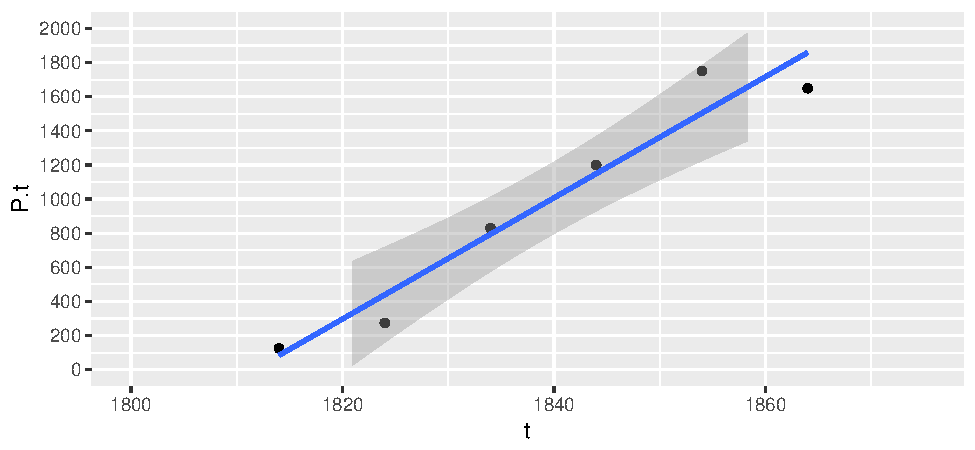
\includegraphics{Christophe_Hunt_hw10_files/figure-latex/unnamed-chunk-3-1.pdf}

\begin{quote}
Based on the above graph I would estimate the population limit at \(M\)
= 1900.
\end{quote}

\subsection{\texorpdfstring{b. Plot ln{[}P/(M-P){]} against \(t\). If a
logistic curve seems reasonable, estimate \(rM\) and
\(t\)*.}{b. Plot ln{[}P/(M-P){]} against t. If a logistic curve seems reasonable, estimate rM and t*.}}\label{b.-plot-lnpm-p-against-t.-if-a-logistic-curve-seems-reasonable-estimate-rm-and-t.}

\begin{Shaded}
\begin{Highlighting}[]
\NormalTok{M <-}\StringTok{ }\DecValTok{1900}
\NormalTok{ln.p <-}\StringTok{ }\KeywordTok{log}\NormalTok{(P.t/(M -}\StringTok{ }\NormalTok{P.t))}
\NormalTok{df2 <-}\StringTok{ }\KeywordTok{as.data.frame}\NormalTok{(}\KeywordTok{cbind}\NormalTok{(t,ln.p))}
\end{Highlighting}
\end{Shaded}

\begin{Shaded}
\begin{Highlighting}[]
\KeywordTok{ggplot}\NormalTok{(df, }\KeywordTok{aes}\NormalTok{(}\DataTypeTok{x =} \NormalTok{t, }\DataTypeTok{y =} \NormalTok{ln.p)) +}
\StringTok{  }\KeywordTok{geom_point}\NormalTok{() +}
\StringTok{  }\KeywordTok{stat_smooth}\NormalTok{(}\DataTypeTok{method =} \StringTok{"lm"}\NormalTok{, }\DataTypeTok{se =} \OtherTok{FALSE}\NormalTok{) +}
\StringTok{  }\KeywordTok{theme_minimal}\NormalTok{()}
\end{Highlighting}
\end{Shaded}

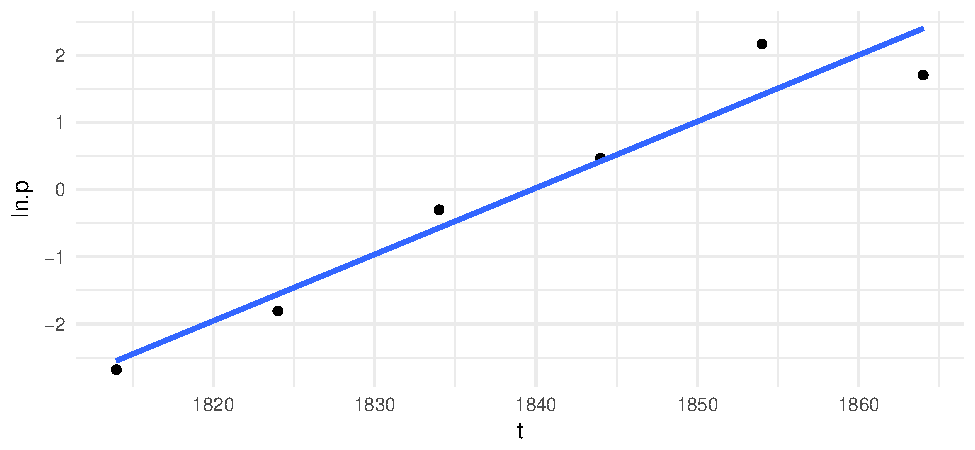
\includegraphics{Christophe_Hunt_hw10_files/figure-latex/unnamed-chunk-5-1.pdf}

\begin{quote}
This graph result does approximate a straight line, thus we accept the
assumptions of logistic growth. Therefore, lets estimate estimate \(rM\)
and \(t\)*.
\end{quote}

\begin{Shaded}
\begin{Highlighting}[]
\NormalTok{rM <-}\StringTok{ }\KeywordTok{lm}\NormalTok{(ln.p ~}\StringTok{ }\NormalTok{t)$coefficients[}\StringTok{"t"}\NormalTok{]}
\end{Highlighting}
\end{Shaded}

\(rM\) = 0.1034121

\begin{quote}
\(t^*\) follows this equation: \(t* = \frac{-C}{rM}\)
\end{quote}

\begin{Shaded}
\begin{Highlighting}[]
\NormalTok{C <-}\StringTok{ }\KeywordTok{log}\NormalTok{(P.t[}\DecValTok{1}\NormalTok{]/(M -}\StringTok{ }\NormalTok{P.t[}\DecValTok{1}\NormalTok{]))-rM}
\StringTok{`}\DataTypeTok{t*}\StringTok{`} \NormalTok{<-}\StringTok{ }\KeywordTok{as.numeric}\NormalTok{(-C/rM) +}\StringTok{ }\NormalTok{t[}\DecValTok{1}\NormalTok{]}
\StringTok{`}\DataTypeTok{t*}\StringTok{`} 
\end{Highlighting}
\end{Shaded}

\begin{verbatim}
## [1] 1840.657
\end{verbatim}

\(t^*= 1841\)

\newpage

\section{Page 478: problem 6}\label{page-478-problem-6}

Suggest other phenomena for which the model described in the text might
be used.

\begin{quote}
Ancedontally, I understand that a major utility cost of a building is
the heating and cooling. Administering the correct ``dosage'' of heated
air or cooled air to maintain a constant comfortable temparture would be
a fiscal and pyschological benefit. By using the model it seems possible
to tune the air volume to correct the internal temperature in the most
effecient manner.
\end{quote}

\section{Page 522: problem 21}\label{page-522-problem-21}

Oxygen flows through a tube into a liter flask filled with air, and the
mixture of oxygen and air (considered well stirred) escapes through
another tube. Assuming that air contains 21\% oxygen, what percentage of
oxygen will the flask contain after 5 L have passed through the intake
tube?

\begin{quote}
Reframing the question, 100\% Oxygen is flowing into a liter flask that
is currently filled at 21\% oxygen and 79\% air, as the mixture leaves
the liter flask the air is being replaced by oxygen so we are interested
in the change in the volume of oxygen in the liter flask. We are further
interested in the total oxygen volume after 5L has been passed through
the 1L flask.
\end{quote}

\(V'C_r = V'C + V_r + V_r \frac{dC}{dt}\)

\(Cr = 1, C_0 = .21, V_r = 1\)

\(\frac{V^1}{V_r}t = ln\frac{C_r-C}{C_r-C_0} = ln\frac{1-C}{1-0.21}\)

\(C = 1 - 0.79e^{\frac{-v^1t}{v_r}}\)

\begin{Shaded}
\begin{Highlighting}[]
\NormalTok{C <-}\StringTok{ }\DecValTok{1} \NormalTok{-}\StringTok{ }\FloatTok{0.79}\NormalTok{*}\KeywordTok{exp}\NormalTok{(-}\DecValTok{5}\NormalTok{)}
\NormalTok{C}
\end{Highlighting}
\end{Shaded}

\begin{verbatim}
## [1] 0.994677
\end{verbatim}

The total volume of oxygen after 5L has passed through a 1L flask is
99.5\%


\end{document}
